% !TeX root = ../main.tex
In questo capitolo viene descritto un caso d'uso aziendale di sviluppo di applicazione mobile adottando i metodi, gli automatismi e gli strumenti descritti nel capitolo \ref{ch:ch4}. L'obiettivo è quello di dimostrare l'efficacia del modello progettato tramite lo sviluppo di una applicazione mobile per la gestione e la visualizzazione dei contenuti digitali pubblicati da Maggioli SpA in formato ebook e rilasciata per le piattaforme Android e iOS.

\section{Analisi dei Requisiti}
\subsection{Requisiti Funzionali}
\begin{itemize}
    \item \textbf{R1} - Visualizzare documenti.
    \begin{itemize}
        \item \textbf{R1.1} - In modo fluido, mostrando il contenuto adattato al dispositivo in cui viene mostrato.
        \item \textbf{R1.2} - In modo statico, mostrando il contenuto con uno specifico layout indipendente dal dispositivo in cui viene mostrato.
    \end{itemize}
    \item \textbf{R2} - Modificare documenti in modo fluido (lato utente).
    \begin{itemize}
        \item \textbf{R2.1} - Aggiungere commenti, sottolineature, evidenziazioni, al contenuto fluido.
        \item \textbf{R2.2} - Memorizzare commenti, sottolineature, evidenziazioni apportate al contenuto fluido.
    \end{itemize}
    \item \textbf{R3} - Gestione utente.
    \begin{itemize}
        \item \textbf{R3.1} - Login (autenticazione) utente.
        \item \textbf{R3.2} - Visualizzare documenti a cui l'utente è abbonato.
    \end{itemize}
    \item \textbf{R4} - Ricerca documenti
    \begin{itemize}
        \item \textbf{R4.1} - Ricerca documenti senza autenticazione. Qualsiasi utente può effettuare una ricerca dei documenti disponibili, senza ottenere il contenuto.
        \item \textbf{R4.2} - Ricerca avanzata in base a diversi campi. %TODO: da definire quali campi
    \end{itemize}
    \item \textbf{R5} - Convertire documenti da modo statico a modo fluido.
    \item \textbf{R6} - Modificare documenti in modo fluido (lato azienda).
    \begin{itemize}
        \item \textbf{R6.1} - Aggiungere elementi/contenuti al documento in modo fluido (hyperlink, quiz, video, immagini, ...). %TODO: definire quali cose sono da aggiungere al documento
        \item \textbf{R6.2} - Memorizzare gli elementi/contenuti apportati al documento in modo fluido (hyperlink, quiz, video, immagini, ...).
    \end{itemize}
\end{itemize}

\subsection{Requisiti Non Funzionali/Tecnologici}
\begin{itemize}
    \item \textbf{T1} - Applicazione nativa Android e iOS, sfruttando Kotlin Multiplatform Mobile (KMM).
    \item \textbf{T2} - Continuous Integration e Continuous Delivery
    \begin{itemize}
        \item \textbf{T2.1} - Analisi statica del codice (SAST\footnote{Static Application Security Testing}).
        \item \textbf{T2.2} - Unit testing, code coverage e E2E\footnote{End-to-End} testing.
        \item \textbf{T2.3} - Rilascio automatico nei relativi store delle piattaforme scelte (Google Play per Android e App Store per iOS).
    \end{itemize}
    \item \textbf{T3} - Monitoraggio applicazione (Analytics).
\end{itemize}

\begin{figure}[H]
\centering
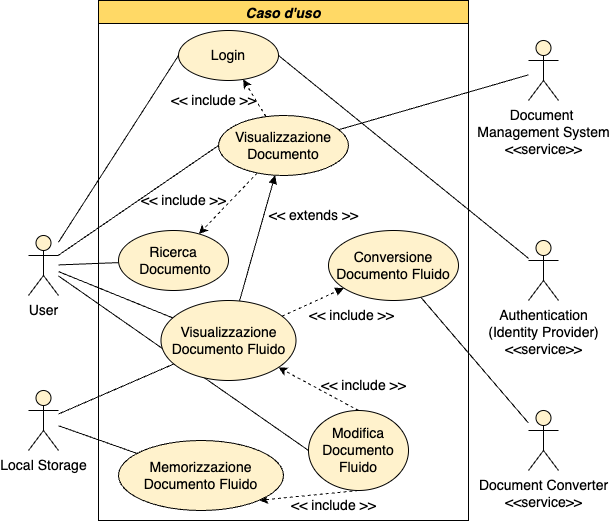
\includegraphics[width=1\textwidth]{img/tesi-1-Use-case.drawio.png}
\caption{Diagramma dei casi d'uso: funzioni/servizi offerti dal sistema Ebook App PoC}
\end{figure}

\begin{figure}[H]
\centering
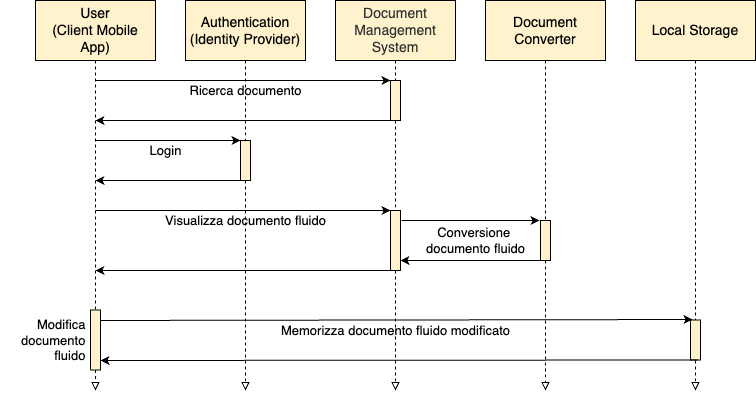
\includegraphics[width=1\textwidth]{img/tesi-2-Use-case2.drawio.png}
\caption{Diagramma di sequenza: scenario di modifica di un nuovo documento "fluido"}
\end{figure}


\section{Analisi Formati Digitali Fluidi}
I documenti attualmente sono reperibili in formato PDF e/o HTML. Il formato PDF è quello con cui i documenti vengono effettivamente archiviati: per ottenere un documento in formato HTML è necessario utilizzare un servizio interno, chiamato \textit{pdf2html}, il quale effettua la conversione. Entrambi i formati rispettano i requisiti per i documenti definiti "statici" ma non per quelli definiti "fluidi":
\begin{itemize}
    \item \textbf{PDF} (Portable Document Format) - Formato di file sviluppato da Adobe per rappresentare documenti di testo e immagini in modo indipendente dall'hardware e dal software utilizzati per generarli o per visualizzarli. Viene dunque generato e visualizzato con uno specifico layout.
    \item \textbf{HTML} (HyperText Markup Language) - Linguaggio di formattazione che descrive le modalità di impaginazione o visualizzazione grafica (layout) del contenuto, testuale e non, di una pagina web attraverso tag di formattazione. Viene generato tramite conversione del documento PDF riportando fedelmente il layout iniziale.
\end{itemize}
Per soddisfare i requisiti \textit{R1.1}, \textit{R2.1}, \textit{R5} e \textit{R6.1} il formato "fluido" deve:
\begin{itemize}
    \item rappresentare solamente il contenuto dei documenti "statici", rimuovendo tutte le formattazioni di layout,
    \item essere modificabile,
    \item poter essere ricavato convertendo un documento attualmente in formato "statico" (ovvero deve esistere un algoritmo/software per poter effettuare la conversione).
\end{itemize}
I formati attualmente disponibili che soddisfano i requisiti sopra indicati rappresentano implementazioni dello standard Open eBook (OeB), elaborato dall'Open E-book Forum. Tra questi i formati più diffusi sono:
\begin{itemize}
    \item \textbf{MOBI} (Mobipocket) - Standard proprietario (\textit{Amazon}) per la pubblicazione di libri digitali (eBook).\\
    Principali caratteristiche:
    \begin{itemize}
        \item basato sulla Open eBook standard utilizzando XHTML,
        \item annotazioni (highlights, segnalibri, correzioni, note e disegni) possono essere applicati, organizzati, e richiamati,
        \item può includere anche JavaScript e cornici.
    \end{itemize}
    \item \textbf{EPUB} (Electronic Publication) - Standard aperto specifico per la pubblicazione di libri digitali (eBook).\\
    Principali caratteristiche:
    \begin{itemize}
        \item basato sulla Open eBook standard utilizzando XML,
        \item a partire da settembre 2007 è lo standard ufficiale dell'International Digital Publishing Forum (IDPF)\footnote{\url{https://web.archive.org/web/20080827131750/http://www.idpf.org/2007/ops/OPS_2.0_final_spec.html}},
        \item CSS per il layout e la formattazione,
        \item testo "re-flowable" con grafica raster e vettoriale,
        \item disponibilità di diversi software, sia proprietari che open source, per la manipolazione del file (\textit{Adobe InDesign}, \textit{Sigil}, \textit{Calibre}, ...),
        \item disponibilità di tante librerie in diversi linguaggi per la manipolazione del file.
    \end{itemize}
\end{itemize}
Le caratteristiche determinanti che hanno portato alla scelta del formato EPUB sono state (\textit{i}) lo standard aperto e (\textit{ii}) la disponibilità, sia di software che di librerie, per la manipolazione del file. 

\section{Progettazione}
In questa sezione viene descritta la fase di progettazione del sistema, le cui attività principali consistono nella ($i$) modellazione del dominio e ($ii$) nella progettazione dell'interfaccia grafica tramite mockup.

\subsection{Modellazione Dominio}

L'obiettivo principale della applicazione è quello di permettere all'utente di "sfogliare" i contenuti digitali offerti da Maggioli sul proprio dispositivo. In questo caso si identificano quindi tre contesti:

\begin{itemize}
    \item \textit{Reader} (Core) - Contesto principale del progetto. Racchiude tutti gli aspetti con maggiore valore per l'utente riguardanti la lettura e personalizzazione dei contenuti digitali. 
    \item \textit{Sisred} - Rappresenta il contesto della sorgente dei contenuti digitali Maggioli (Sistema Redazionale\cite{amslaurea23043}). In questo contesto non esistono i concetti di \textit{favorite}, \textit{highlight}, \textit{bookmark} e \textit{progression} mentre è condiviso il concetto di libro e utente.
    \item \textit{User} - Contesto che definisce tutti gli aspetti a riguardo degli utenti. In questo contesto esiste il solo concetto di utente, il quale è condiviso con gli altri contesti.
\end{itemize}

\begin{figure}[H]
\centering
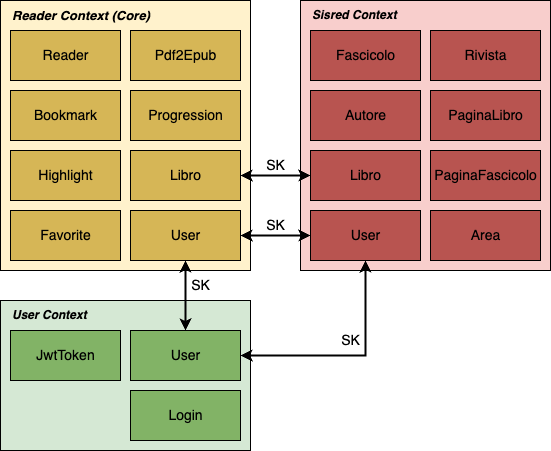
\includegraphics[width=0.8\textwidth]{img/tesi-20-app-domain.drawio.png}
\caption{Context Map: panoramica globale dei contesti del progetto e delle relazioni che intercorrono tra di essi}
\end{figure}

Tra i contesti definiti esistono delle relazioni di tipo \textit{Shared Kernel}\cite{evans_domain-driven_2004} (SK) con l'obiettivo di evitare duplicazioni e semplificare l'integrazione. Relazioni di questo tipo consistono nella condivisione di un sottoinsieme del dominio modellato, che corrisponde tipicamente al dominio core. Un esempio di relazione SK è l'utilizzo di codice o schemi DB condivisi\footnote{\url{https://github.com/ddd-crew/context-mapping}}.\\

Per la modellazione del dominio si fa uso dei seguenti concetti\cite{evans_domain-driven_2004}:
\begin{itemize}
    \item \textit{Entity} - Oggetto definito dalla sua identità e non dai suoi attributi. Ogni libro è univoco, identificato da uno specifico codice, chiamato ISBN\footnote{International Standard Book Number}.
    \item \textit{Value Object} - Al contrario delle entità, questi oggetti sono definiti dai loro attributi e non hanno una identità concettuale ma servono a descrivere alcune caratteristiche di un oggetto. Un esempio è il segnalibro: ciò che è rilevante è la pagina del libro che esso referenzia e non la sua identità.
    \item \textit{Aggregate} - Insieme di oggetti legati da una entità padre chiamata \textit{Root} (radice di aggregazione). L'aggregato composto da \textit{Bookmark}, \textit{Highlight}, \textit{Progression}, \textit{Favorite} ha come radice l'entità \textit{Libro}.
    \item \textit{Service} - Operazione che non appartiene logicamente a nessun oggetto. In questo caso la conversione di formato non appartiene alla sola entità libro ma appartiene invece a qualsiasi documento che è possibile convertire.
    \item \textit{Repository} - Oggetto per il recupero di altri oggetti di dominio e per la gestione del loro ciclo di vita. Le entità \textit{User} e \textit{Libro} sono esempi di oggetti di dominio che necessitano di un repository. Permette di disaccoppiare applicazione e domain design dalle specifiche tecnologie/strategie di persistenza come multipli database e datasource (locali e/o remoti).
\end{itemize}

\begin{figure}[H]
\centering
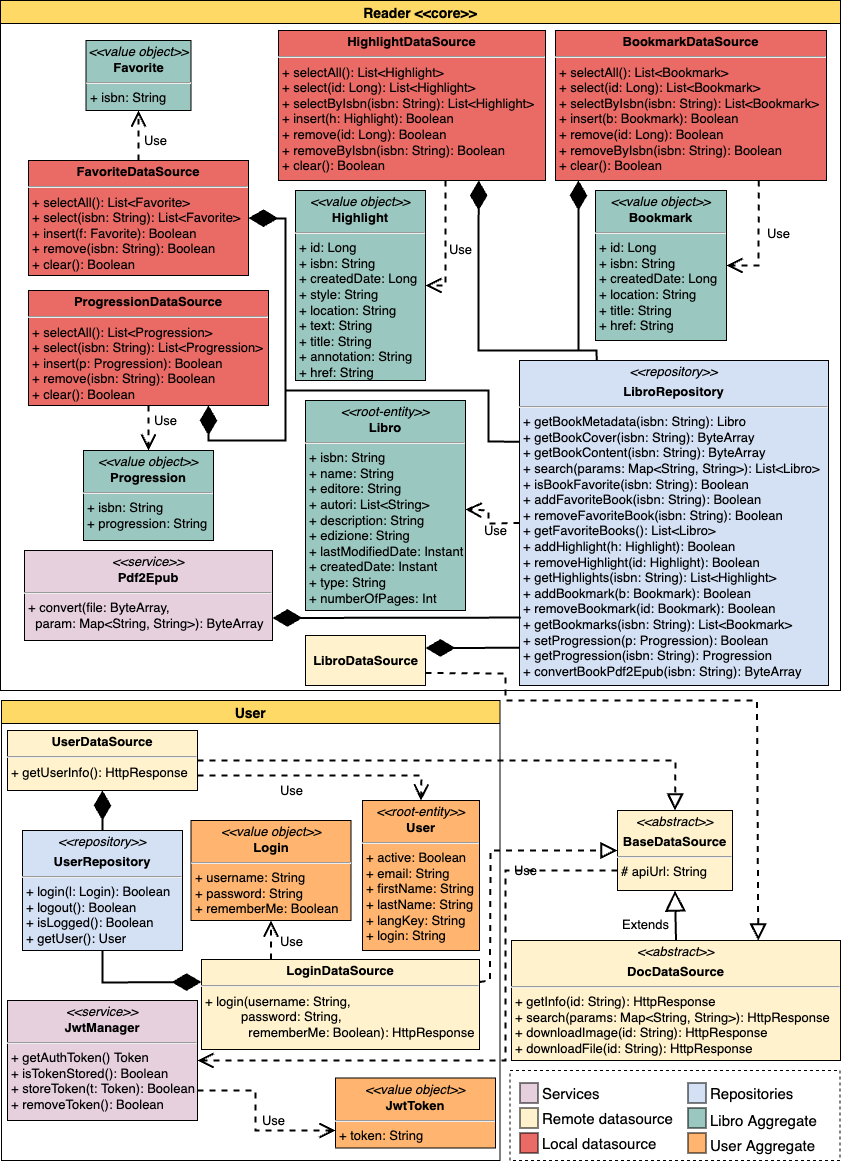
\includegraphics[width=0.92\textwidth]{img/tesi-25-ddd.drawio.png}
\caption{UML - Diagramma delle classi: Reader Core Domain e User Subdomain}
\end{figure}

\subsection{Progettazione UI}

L'interfaccia grafica della applicazione è stata progettata tramite l'utilizzo di mockup digitali realizzati con il tool grafico open source Drawio\footnote{\url{https://github.com/jgraph/drawio}}. 

\begin{figure}[H]
\centering
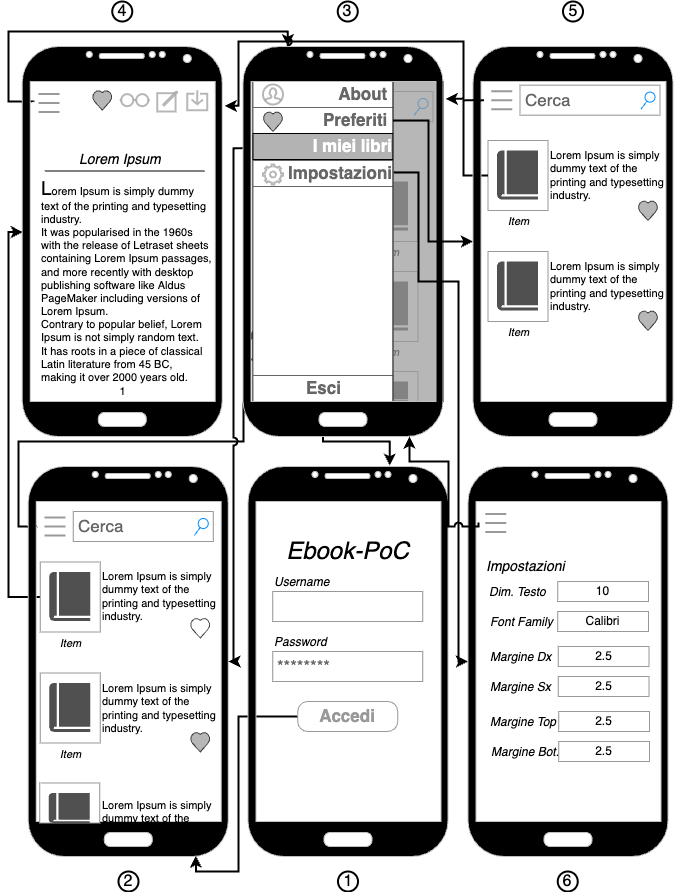
\includegraphics[width=0.8\textwidth]{img/tesi-14-mockup1.drawio.png}
\caption{Alcuni dei mockup realizzati per la progettazione e la validazione della UI (v1)}
\end{figure}

Considerando l'utilizzo tipico di una applicazione della stessa tipologia di quella che deve essere realizzata, sono stati utilizzati alcuni standard de-facto come ad esempio il menu laterale a scomparsa (mockup 4), icona "hamburger" per l'apertura del menu (mockup 3), elenco di elementi con scroll infinito verticale (schermata 5-6), barra di ricerca nella parte alta con icona "lente di ingrandimento" (schermata 2-5-6), ... .

\begin{figure}[H]
\centering
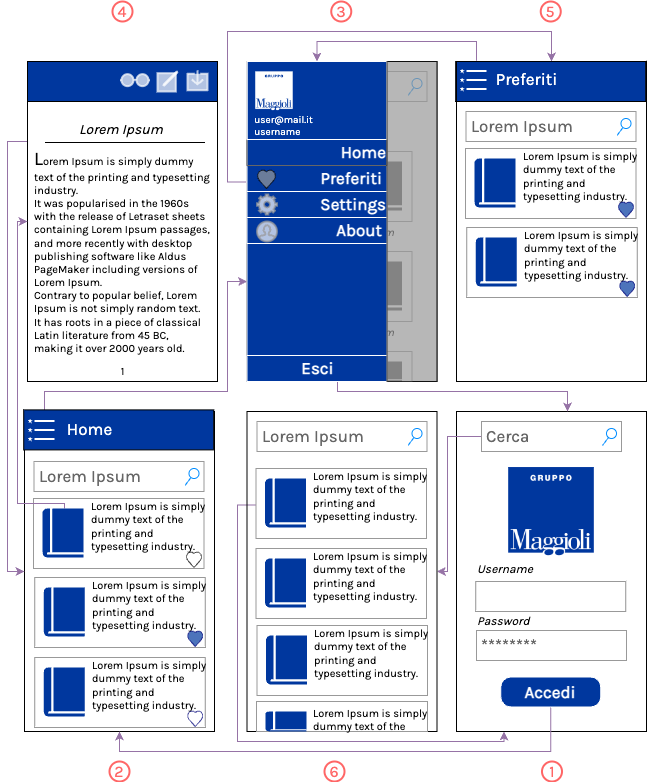
\includegraphics[width=0.8\textwidth]{img/tesi-23-mockupv2.drawio.png}
\caption{Modifiche apportate ai mockup per ottenere la validazione della UI (v2)}
\end{figure}

Sono state necessarie due iterazioni di validazione dei mockup da parte degli interessati per definire l'interfaccia utente desiderata con alcuni vincoli caratteristici del brand Maggioli, come ad esempio l' utilizzo del colore blu \#00379E come colore primario, l'utilizzo del font Karla\footnote{\url{https://github.com/googlefonts/karla}} e la presenza del logo Maggioli. Le schermate necessarie sono quindi:
\begin{itemize}
    \item \textit{Reader} - Schermata responsabile della visualizzazione del contenuto digitale in formato EPUB.
    \item \textit{Login} - Schermata iniziale responsabile alla autenticazione dell'utente.
    \item \textit{Home} - Schermata principale responsabile alla visualizzazione dei contenuti digitali a cui l'utente è autorizzato ad accedere.
    \item \textit{Preferiti} - Schermata responsabile alla visualizzazione dei contenuti digitali preferiti dall'utente.
    \item \textit{Impostazioni} - Schermata responsabile alla visualizzazione e modifica delle impostazioni.
    \item \textit{About} - Schermata responsabile alla visualizzazione di informazioni generali come versione della applicazione, autore, copyright, ... .
    
\end{itemize}

\section{Implementazione}

\subsection{Ricerca Librerie}
Definiti i requisiti e modellato il dominio sono state individuate le seguenti librerie, suddivise per modulo, a supporto dello sviluppo della applicazione:
\begin{itemize}
    \item \textit{Shared}
    \begin{itemize}
        \item \textit{Ktor} - Framework asincrono per lo sviluppo di microservizi e applicazioni web. Nel progetto Ktor è utilizzato per la parte di networking come client HTTP.
        \item \textit{Kotlinx-Serialization} - Libreria multiplatform per la serializzazione dei dati.
        \item \textit{Kotlinx-Datetime} - Libreria multiplatform per la gestione delle date e del tempo.
        \item \textit{Kvault}\footnote{\url{https://github.com/Liftric/KVault}} - Libreria multiplatform per la persistenza dei dati sicura in formato chiave-valore. Tramite una unica API si comporta come wrapper di Keychain, nel caso iOS, e SharedPreferences nel caso Android.
        \item \textit{Koin}\footnote{\url{https://github.com/InsertKoinIO/koin}} - Dependency Injection framework multiplatform.
        \item \textit{Napier}\footnote{\url{https://github.com/AAkira/Napier}} - Logging framework multiplatform.
    \end{itemize}
    \item \textit{Android}
    \begin{itemize}
    \item \textit{Readium} (Kotlin-toolkit)\footnote{\url{https://github.com/readium/kotlin-toolkit}} - Libreria per la manipolazione e visualizzazione di contenuti editoriali digitali. Implementazione specifica per la piattaforma Android. 
    \end{itemize}
    \item \textit{iOS}
    \begin{itemize}
    \item \textit{Readium} (Swift-toolkit)\footnote{\url{https://github.com/readium/swift-toolkit}} - Libreria per la manipolazione e visualizzazione di contenuti editoriali digitali. Implementazione specifica per la piattaforma iOS. 
    \item \textit{KMPNativeCoroutines}\footnote{\url{https://github.com/rickclephas/KMP-NativeCoroutines}} - Libreria che permette l'utilizzo delle coroutine Kotlin in Swift in applicazioni Kotlin Multiplatform.
    \end{itemize}
\end{itemize}

\subsection{Readium}
Tra le librerie individuate quella fondamentale per il dominio applicativo è \textit{Readium}.
La necessità di un tool open-source, robusto e performante per la manipolazione e la lettura di formati editoriali digitali è alla base del progetto Readium. Essa infatti consiste in un insieme di toolkit per diversi formati (come epub, audiolibri e libri image-based) e diverse piattaforme (Android, iOS, Desktop e Web).\\
\begin{figure}[H]
\centering
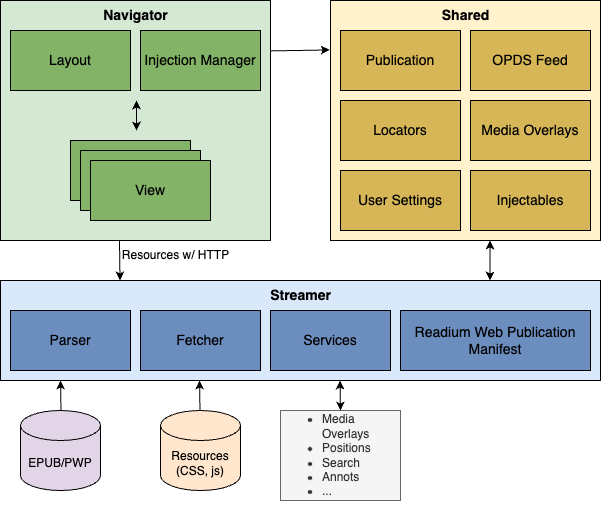
\includegraphics[width=1\textwidth]{img/tesi-22-readiumarch.drawio.png}
\caption{Architettura libreria Readium}
\end{figure}
Readium è composto da quattro moduli principali:
\begin{itemize}
    \item \textit{Publication Server} - Fornisce le pubblicazioni tramite un server locale HTTPS.
    \item \textit{Streamer} - Modulo composto dai seguenti due sottomoduli:
    \begin{itemize}
        \item \textit{Parser} - Responsabile del parsing delle pubblicazioni e della loro esposizione utilizzando un modello in-memory.
        \item \textit{Fetcher} - Si occupa di ottenere i contenuti delle pubblicazioni e della loro manipolazione (in particolare injection di CSS e Javascript nelle risorse HTML).
    \end{itemize}
    \item \textit{Navigator} - Utile alla navigazione delle risorse di una pubblicazione secondo diverse strategie basate sulla natura della pubblicazione (ebook, audiolibri, ...). Interagisce con il modulo \textit{Streamer} per utilizzare il modello in-memory o per ottenere manifesto JSON attraverso il modello condiviso (\textit{Shared}).
\end{itemize}

% parlare della implementazione del modulo shared e della strategia expect/actual adottata
\begin{figure}[H]
\centering
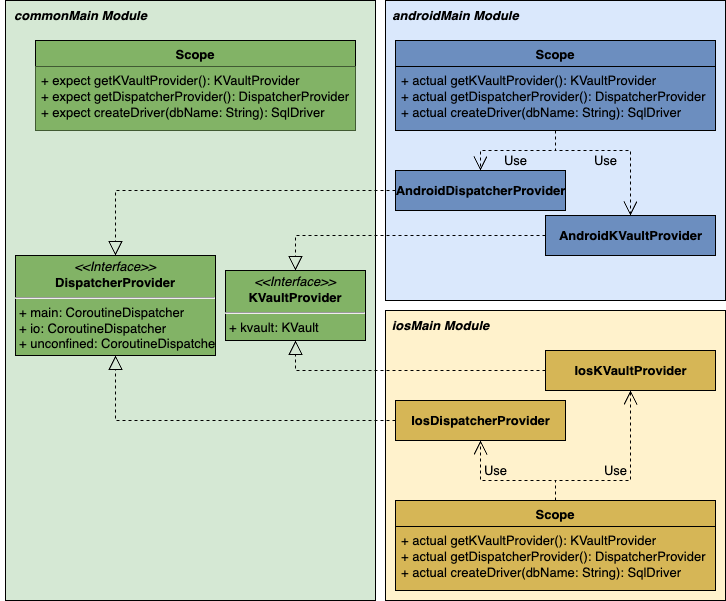
\includegraphics[width=1\textwidth]{img/tesi-21-expectactual.drawio.png}
\caption{Strategia \textit{Expect/Actual} adottata per l'implementazione dei servizi infrastrutturali specifici delle piattaforme, persistenza e concorrenza, sfruttando la tecnica \textit{dependency injection}}
\end{figure}

NavigationController e navigation graph per gestire il flusso tra i vari fragment della app. La fragment home è quella principale e prima di essere creata, se l'utente non ha fatto login, viene rediretto\footnote{\url{https://developer.android.com/guide/navigation/navigation-conditional}} al fragment di login per farlo autenticare e poi riportato indietro alla schermata di home (popStackBack)
\footnote{\url{https://medium.com/swlh/android-navigation-component-part-1-6191323eaf39}}.

Utilizzo di PagingData (Paging 3) per scaricare on demand il contenuto e mostrarlo nel recycler view con lo scroll.

Per poter gestire la persistenza nel shared è necessario gestire tipi di dato primitivi (e.g. String): per questo nel db vengono salvati solo string e sulle due piattaforme sono stati aggiunti metodi per fare il toString degli oggetti di readium (esempio locator: ogni volta che lo devo memorizzare faccio json.toString e ogni volta che cerco i dati faccio Locator.fromJson(Json.fromString(risultatoQuery)))